% !TEX root =  ../main.tex
\chapter{Synthèse d'un régulateur discret}

\section{Introduction}
Durant la troisième et dernière séance de laboratoire, il a été demandé aux élèves de synthétiser sur le logiciel MATLAB\textregistered{} un régulateur discret de compensation en boucle fermée et d'en analyser la réponse.
Pour ce faire, il a tout d'abord fallu calculer l'équivalent échantillonné bloqué de ce régulateur (discrétisation).
Et ensuite, imposer un intégrateur dans le régulateur discret de compensation.

\section{Hypothèses}
Soit le système défini par l'équation :
\begin{equation}
	H_c(s) = \frac{1}{s\left( s+0,5\right)}
		   = \frac{2}{s\left(2s+1  \right)}
	\label{eqn:system3}
\end{equation}
Nous cherchons à effectuer la synthèse d'un régulateur discret compensant le système~(\ref{eqn:system3}) en boucle fermée, et respectant les spécifications suivantes :
\begin{enumerate}
	\item Dépassement de 5\% $(\xi=0,69)$
	\item Temps de réponse à 95\% ($3T$) de 1
	\item Erreur de vitesse nulle
	\item $h = 0,1$
\end{enumerate}
Notons avant tout que la spécification sur l'erreur de vitesse nulle implique un double intégrateur dans la chaîne directe.
Ceci nous indique d'avance que le régulateur suivra la forme :
\begin{equation}
	R(Z) = \frac{\dots}{(Z-\alpha)(Z-\beta)}
\end{equation}

%%%%%%%%%%%%%%%%%
\section{Analyse}
La première étape est toujours la même, nous devons traduire la fonction de transfert dans le domaine discret.
Pour cela nous utilisons la commande \texttt{c2d()} de MATLAB\textregistered{} qui équivaut à convoluer la fonction par un bloqueur d'ordre 1.
C.-à-d. effectuer l'opération :
\begin{align}
	H_d(Z) &= \underset{s\rightarrow Z}{\mathcal{L}} H_c(s) \\[2mm]
		   &= \frac{k}{(Z-1)(Z-p)}
		   \label{eqn:uncompensated}
\end{align}
Dans cette forme, les points sont distants de la période d'échantillonnage.
Cela entraine que l'influence de l'entrée sur la sortie est perçue après cette même période.
Ceci implique également que la différence entre l'ordre du dénominateur et du numérateur doit être égale à 1.
Pour imposer cet ordre, nous rajoutons un zéro au numérateur de~(\ref{eqn:uncompensated}).
Ce qui donne :
\begin{equation}
	H_d(Z) = \frac{k\,(Z-z)}{(Z-1)(Z-p)}
\end{equation}

De cette forme discrétisée, nous désirons extraire les pôles et les zéros.
MATLAB\textregistered{} propose une fonction permettant de les extraire en un appel, \texttt{zpkdata()}.
Nous employons par la suite ces coefficients obtenus dans le régulateur $R(Z)$ pour compenser $H_d(Z)$.
$R(Z)$ est donc une régulateur de compensation.

\begin{equation}
	R(Z) = k\,\frac{(Z-p)}{(Z-z)(Z-1)}
\end{equation}
On a un décalage car l'ordre du dénominateur est plus grand que l'ordre du numérateur.
Quand le régulateur aperçoit un écart de réglage à sa consigne, il doit réagir immédiatement.
Il \og{}mouline\fg{} dans un temps qui est supposé très petit et négligeable sur la période puis il envoie.
On rajoute un zéro au numérateur pour faire en sorte qu'il n'y ait pas de retard dans le régulateur.
\begin{equation}
	R(Z) = k\,\frac{(Z-p)(Z-n)}{(Z-z)(Z-1)}
\end{equation}
Ensuite nous faisons le produit en boucle ouverte du régulateur avec le système.
\begin{equation}
	R(Z)H_d(Z) = B_0(Z) = \frac{k\,(Z-n)}{(Z-1)^2}
\end{equation}
On constate que dans le chaîne directe, il y a bien un retard d'une période.

%%%%%%%%%%%%%%%%%%
\section{Synthèse}

Dans le plan complexe les pôles continus sont sur une droite d'amortissement inclinée d'un certain angle \Theta{}, tel que dans notre cas $sin(\Theta) = 0,69$.
C'est le sin de l'angle d'inclinaison de la droite d'amortissement sur laquelle se trouvent les pôles.
Le $sin(\Theta)$ détermine ainsi le dépassement de 5\% cité dans l'énoncé du laboratoire et qui est une des spécifications du régulateur.

Ensuite, nous avons le temps de réponse à 95\% de 1.
Si nous traduisons cela sous forme de pôles et de zéro dans le cas d'un filtre du 1\up{er} ordre, nous trouvons que le lien entre un pôle et une constante de temps est l'inverse l'un de l'autre.
La constante de temps vaut T=1/3.
La partie réelle du pôle va donc se trouver à l'inverse (et signe opposé) de cette constante de temps.
On peut le voir sur la Figure~\ref{fig:temps-de-reponse} où, comme on l'a dit, $\delta = T^{-1}$ et donc $\delta = 3$.
On trouve ainsi la paire de pôles complexes  qui donne en boucle fermée une réponse pour que les deux premières conditions de l'énoncé soient respectées.

\begin{figure}[!ht]
	\centering
	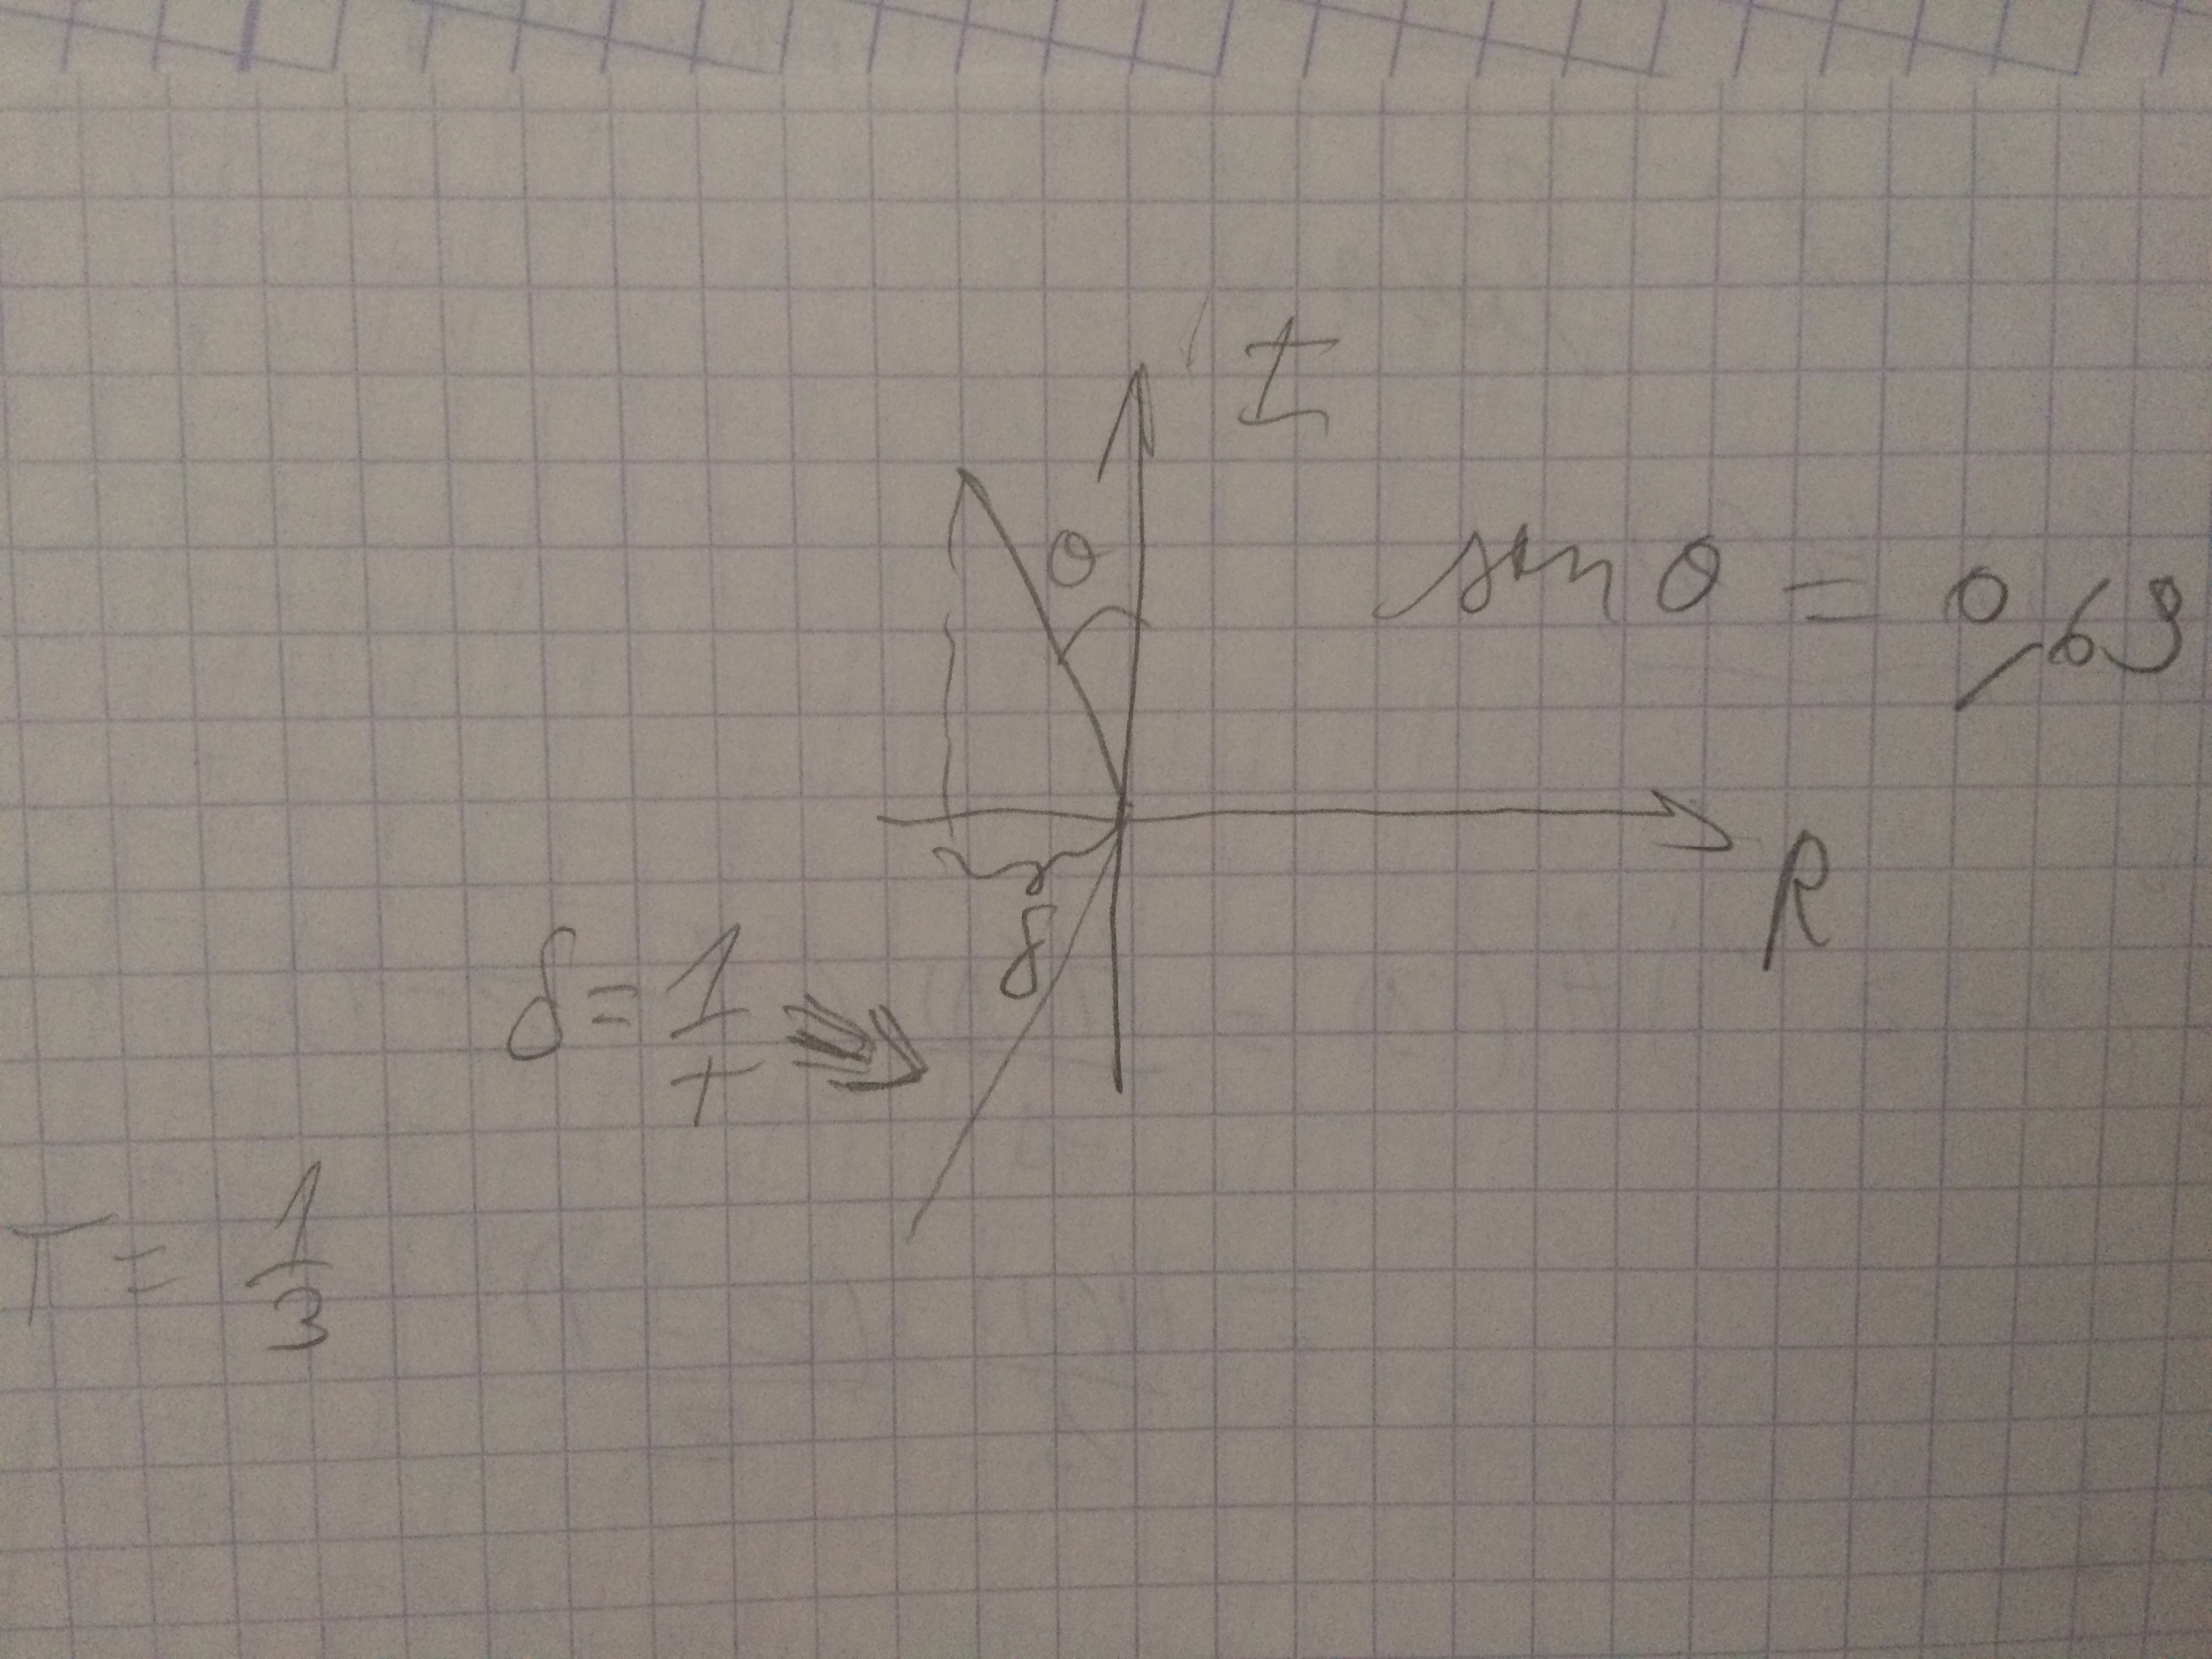
\includegraphics[scale=0.1]{images/IMG_1681.jpg}
	\caption{Temps de réponse.}
	\label{fig:temps-de-reponse}
\end{figure}

Nous pouvons également faire la synthèse du régulateur.
Nous savons que $H_s(Z)$ est sous la forme :
\begin{equation}
	H_s(Z) = \frac{\dots}{(Z-P_{d1})(Z-P_{d2})}
\end{equation}
Nous cherchons à trouver les valeurs de $P_{d1}$ et $P_{d2}$.
Nous allons les trouver par équivalences avec $F(Z)$, la transmittance en boucle fermée.
\begin{equation}
	F(Z) = \frac{k\,(Z-n)}{(Z-1)^2+k\,(Z-n)}
\end{equation}

\begin{equation}
	\begin{cases}
		k = 2-P_{d1}-P_{d2} \\[2mm]
		n = \frac{(1-P_{d1}P_{d2})}{k}
	\end{cases}
	\label{eqn:equivalence}
\end{equation}

En utilisant la fonction \texttt{dtr2ord2o.m} fournie, nous avons pu générer la transmisttance d'un système continu du second ordre répondant aux spécifications.
Nous avons pu extraire les valeurs $P_{d1}$ et $P_{d2}$ de cette transmittance, et par résolution du système~\ref{eqn:equivalence} nous avons obtenu la transmittance du système à synthétiser en boucle fermée.

\pagebreak
Cette séquence d'opération a été réalisé sous MATLAB à l'aide du script suivant :
{\footnotesize\begin{verbatim}
h = 0.1;
nH = 1;
dH = conv([1 0], [1,0.5]);
Hc = tf(nH, dH);
Hd = c2d(Hc, h, 'zoh');

% R(z) = [K(Z-p)(Z-n)]/[(Z-z)(Z-1)]
[z,p,~] = zpkdata(Hd, 'v');
p = p(2);

[pc] = dtr2ord2o(1, 5, 5); % trouve les poles pd1 et pd2
pd = exp(pc*h);            % discretise les poles
K = 2-pd(1)-pd(2);         % calcul le gain d'Evans unite
n = (1-pd(1)*pd(2))/K;     % calcul du zero additionnel

Z = tf('z', h);
F = K*(Z-n)/((Z-1)^2+K*(Z-n));    % boucle fermee
R = K*(Z-p)*(Z-n)/((Z-z)*(Z-1));  % regulateur

% autre maniere de fermer la boucle
Bo = R*Hd;
Bf = feedback(Bo,1);
Bf = minreal(Bf);
\end{verbatim}}


\section{Conclusion}
Une fois les valeurs de $k$ et $n$ obtenues, la fonction de transfert du régulateur $R(Z)$
et la transmittance en boucle fermée $F(Z)$.
Nous pouvons finalement réaliser un modèle simulink pour simuler l'exactitude de nos calculs.
Nous avons tenté de reproduire au mieux l'exemple présenté au laboratoire, notre version est présenté à la figure~\ref{fig:manipulation}.

La partie supérieur du graphique représente l'action correctrice, on note ses oscillations du à la présence d'un zéro dans la partie gauche du cercle des pôles et des zéros.

Dans la partie inférieur du graphique, nous observons tout d'abord l'échelon unitaire en jaune s'exprimant à 0.5 unité de temps.
La courbe en bleu est l'équivalent en $S$ de la fonction $F(Z)$, on peut y noter sa réponse stable avec un très faible dépassement.
Et pour finir en orange se trouve la sortie du système continue $H_c(S)$ qui est placé en cascade à la suite du régulateur $R(Z)$.
On désirait un dépassement de 5\% mais nous obtenons à la place un dépassement monstrueux, cela est dû au zéro que nous avons du ajouter qui entraine également les oscillations de la réponse entre chaque instant d'échantillonnage.
Afficher la sortie du système continue au lieu de $F(Z)$ permet d'observer ces oscillations qui seraient cachées dans l'équivalent échantillonné.

On peut noter que le régulateur effectue correctement sa tâche puisque après une phase de stabilisation et à chaque instant d'échantillonnage, toutes les 0.1 unités de temps, la différence entre la courbe et la valeur attendue est 0 !

\begin{figure}[!ht]
	\centering
	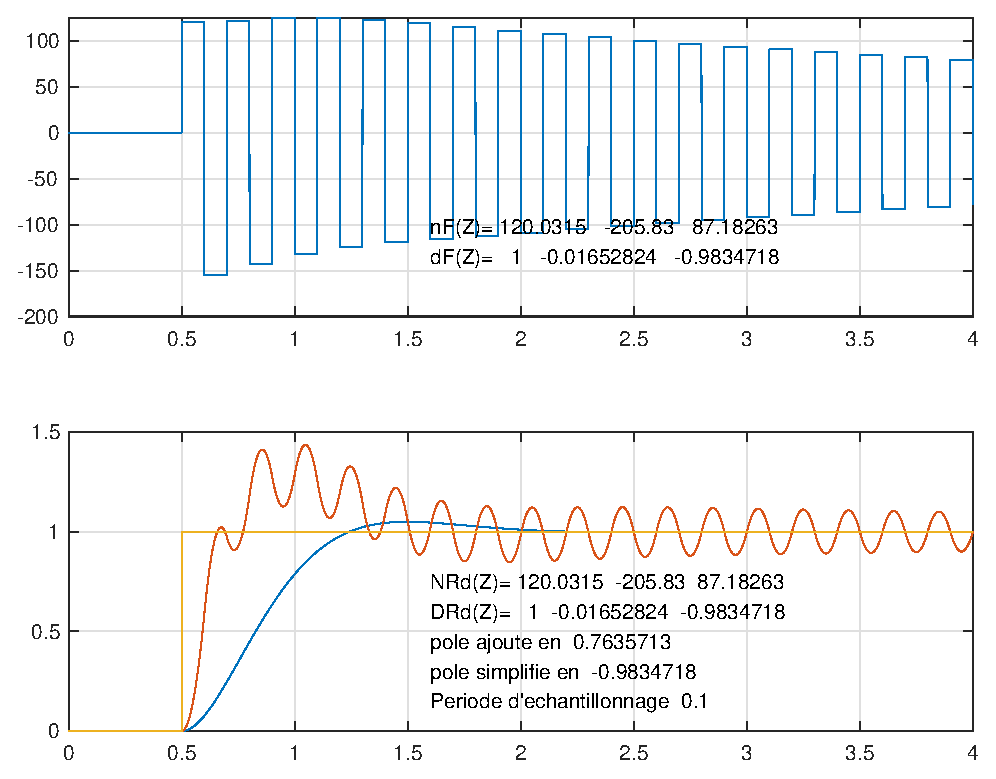
\includegraphics[width=\textwidth]{eps/labo3.eps}
	\caption{Simulation de la transmittance en boucle fermée échantillonnée.
			 On peut apercevoir sur la courbe orange les oscillations de la sortie
			 entre chaque période d'échantillonnage qui dure 100 ms.}
	\label{fig:manipulation}
\end{figure}
